\documentclass[11pt]{article}
\usepackage{dsfont}
\usepackage{amsmath}
\usepackage{graphicx} 
\title{Security Two-Party Computation}
\date{\today}
\author{Feng Wang}
\newcommand{\solution}{\fbox{\textbf{solution}}}
\begin{document}
\maketitle
\paragraph{Part One}{\textbf{A brief introduction to my implementation}}\vspace{2ex}\\
For input $x = x_1x_2\cdots x_n$ and $y= y_1y_2\cdots y_n$, if we want to compute the function 
\begin{align*}
	f(x,y) = \begin{cases}
		&1 \quad x\geq y \\
		&0 \quad x < y
	\end{cases}
\end{align*}
we can compute every bit of $x$ and $y$ from high-order position to low-order position. Firstly we compare $x_1$ with $y_1$, if $x_1 \geq y_1$ then we compare $x_2$ and $y_2$. But if $x_1 < y_1$, we just return 0 since we don't need to care about the remaining bits. Considering the specific function, I'm not trying to implement the whole garbled circuit for $n$ bits numbers. Instead I just consider one bit and construct the garbled circuit for two single bits during every comparison. Because I think it will be faster to yield the result.
\paragraph{Part Two}{\textbf{Garbled circuit}}\vspace{2ex}\\
For two bits 0 and 1, it is easy to get the following table. \\
\begin{center}
\begin{tabular}{c|c|c|c}
	\hline
	a & b & !b & f(a,b) \\
	\hline
	0 & 0 & 1 & 1 \\
	\hline
	0 & 1 & 0 & 0 \\
	\hline 
	1 & 0 & 1 & 1 \\
	\hline
	1 & 1 & 0 & 1 \\
	\hline
\end{tabular} 
\end{center}
\vspace{2ex}
If we only look at $a$ and $!b$, those two and $f(a,b)$ is equivalent to the OR circuit. So the garbled circuit for two bits is,\\
\centerline{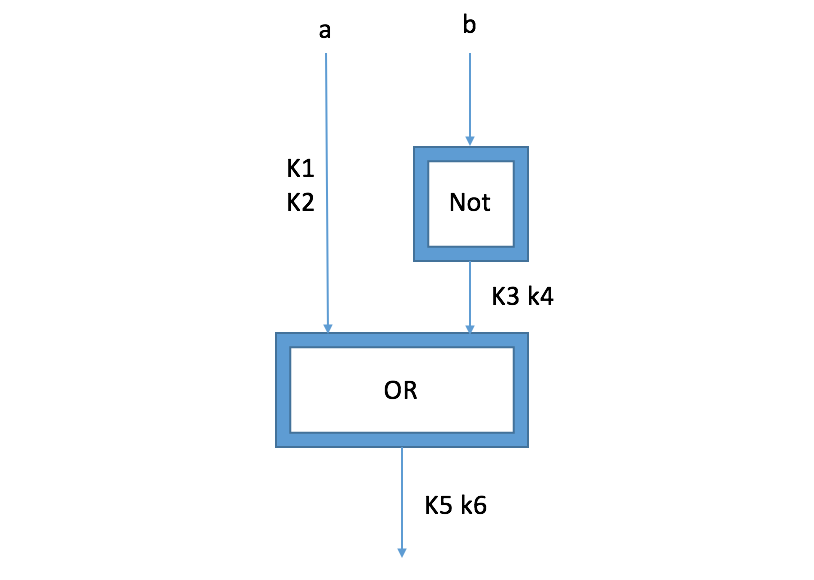
\includegraphics[width=0.6\textwidth]{circuit}}
\paragraph{Part Three}{\textbf{Encryption}}\vspace{2ex}\\
In my implementation, k1,k2,...,k6 are 16-bits generated randomly. I use AES to encrypt each key to be sent because Python already provides AES so it will be easier.
\paragraph{Part Four}{\textbf{Oblivious transfer}}\vspace{2ex}\\
In Bob's side, Bob generates a public key $(N,e)$ and a private key $(N,d)$ using RSA algorithm. Then, he also randomly generates a number $N'$ which has the same length with $N$. If Bob's number is 1 ($b = 1$) now, he may wants to get the key(k3) representing 0 ($!b = 0$). Now, he sends $(N,e)$ and $(N',d)$ to Alice. Alice encrypts k3 and k4 using RSA respectively and sends the results back. So Bob is able to decrypt k3 while fails to decrypt k4 since $N'$ is randomly generated. Apparently, Bob is also able to get k4 without knowing k3 when having 0 in his hand.
\paragraph{Part Five}{\textbf{Achieve the result}}\vspace{2ex}\\
For every comparison, Bob now gets two keys. Suppose Bob now have k2 and k3, which means Alice is 1 and Bob is also 1 now. Since Bob already gets the garbled circuit, which is four-double-encrypted-numbers. Bob use k2 and k3 to decrypt the four numbers and he will achieve four numbers, where only one is either k5 or k6. Bob sends them to Alice. Alice looks at the four numbers and will recognize k6 eventually. Alice will know the result is 1 since k6 represents 1 while Bob doesn't know that. Alice will sent the result to Bob. So both of them will know.
\end{document}